\documentclass{beamer}

\usepackage[utf8]{inputenc}
\usepackage[T1]{fontenc}
\usepackage{graphicx}
\usepackage{hyperref}

\title{Image Embedding for Product Labeling}
\author{Couture Vision}
\date{\today}

\begin{document}

\frame{\titlepage}

\section{Project Objective}
\begin{frame}{Project Objective}

\textbf{Goal:}
\begin{itemize}
    \item Based on a photo of an article, match the reference image of this article.
\end{itemize}

\textbf{Example:}
\begin{columns}
    \column{0.5\textwidth}
    \begin{figure}[t]
        \includegraphics[width=\textwidth]{assets/shoes_test.jpg}
        \caption{Test Image}
    \end{figure}
    \column{0.5\textwidth}
    \begin{figure}[t]
        \includegraphics[width=\textwidth]{assets/shoes_reference.jpeg}
        \caption{Reference Image}
    \end{figure}
\end{columns}

\end{frame}

\begin{frame}{Dataset presentation}
    \begin{itemize}
        \item DAM : 2766 images = 2766 classes
        \item 80 test images without labels
        \item DAM images are clean : regular resolution and proper background
        \item test images : different resolutions, backgrounds; sometimes multiple items in one image.
        \item Basically no training set : we will focus on Siamese network methods : embedding images then comparing embeddings
        \item We (will) manually labelise the test dataset to have an accuracy.
    \end{itemize}
    \end{frame}
    
    \begin{frame}{Test images}
        \begin{figure}
            \includegraphics[width=\textwidth]{assets/p_img.png}
        \end{figure}
    \end{frame}

\section{Introduction}
\begin{frame}{Project Overview}
\begin{itemize}
    \item We utilized Microsoft's ResNet50 and Google's ViT to extract embeddings.
    \item Cosine similarity is used to find the best matches between images.
    \item We preprocess images using \texttt{rembg} to remove backgrounds, as test images (shop pictures) differ from the clean DAM images.
    \item Embedding extraction assists in labeling products by suggesting potential matches.
\end{itemize}
\end{frame}


\section{Methodology}
\begin{frame}{Embedding Extraction Pipeline}
\begin{columns}
    \column{0.5\textwidth}
    \begin{itemize}
        \item Use ResNet50 and ViT to extract image embeddings.
        \item Employ cosine similarity to rank matches.
        \item Preprocess test images with \texttt{rembg} to isolate objects from noisy backgrounds.
    \end{itemize}
    \column{0.5\textwidth}
    \begin{figure}
        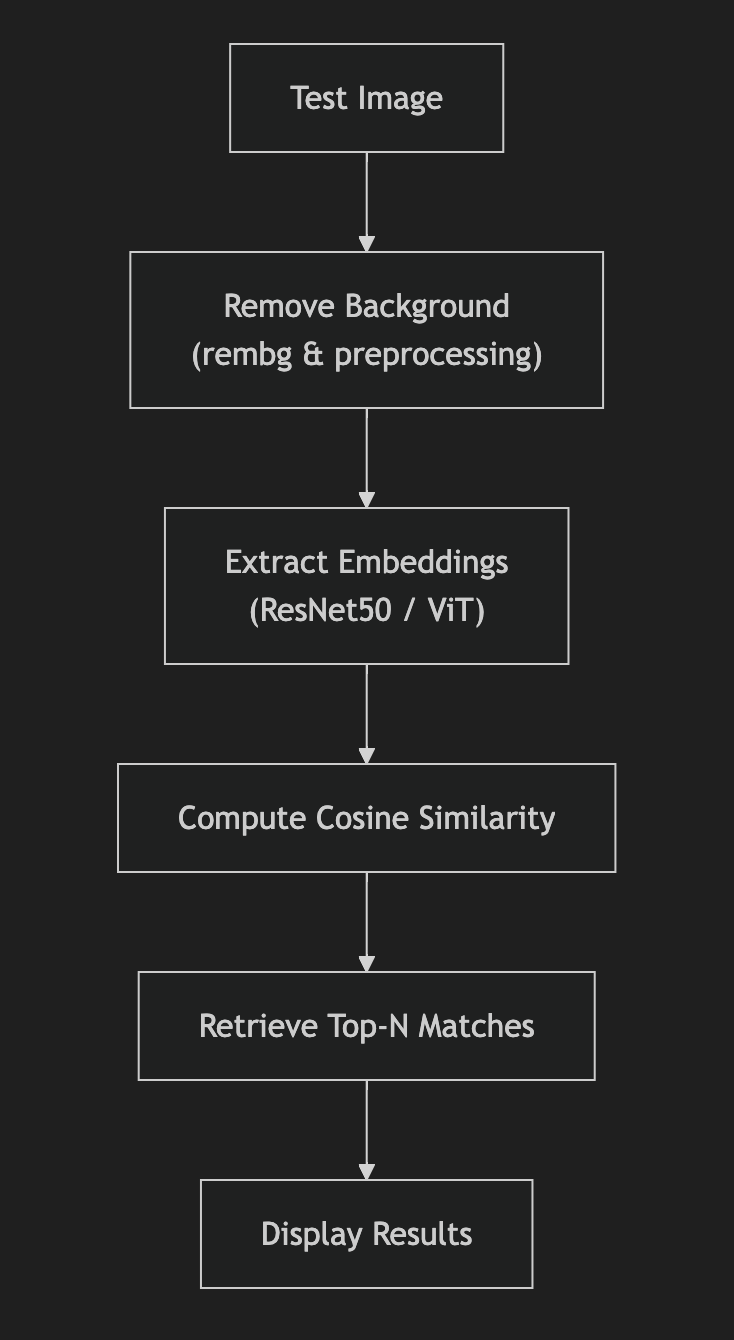
\includegraphics[width=0.6\textwidth]{assets/pipeline_overview.png}
        \caption{Pipeline overview}
    \end{figure}
\end{columns}
\end{frame}

\begin{frame}{Embedding Extraction Pipeline}
    \begin{figure}
        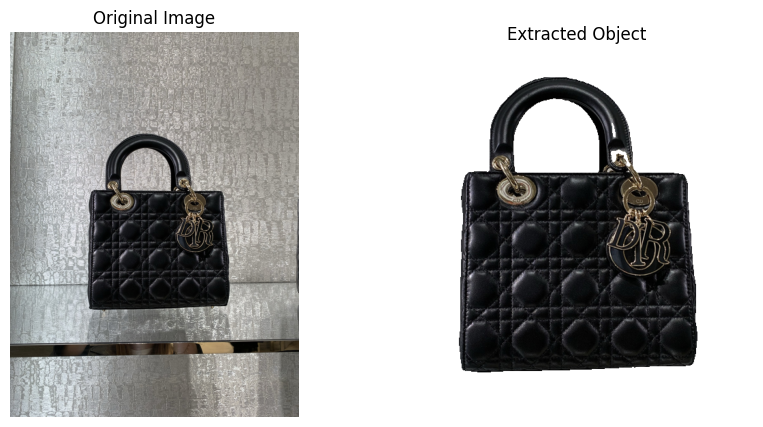
\includegraphics[width=\textwidth]{assets/background_removal.png}
        \caption{Background removal using \texttt{rembg}, scaling and center-cropping}
    \end{figure}
\end{frame}

\begin{frame}{Good Classification Example}
\begin{itemize}
    \item Original image and extracted object.
    \item Top 5 matches with high similarity scores.
\end{itemize}
\begin{figure}
    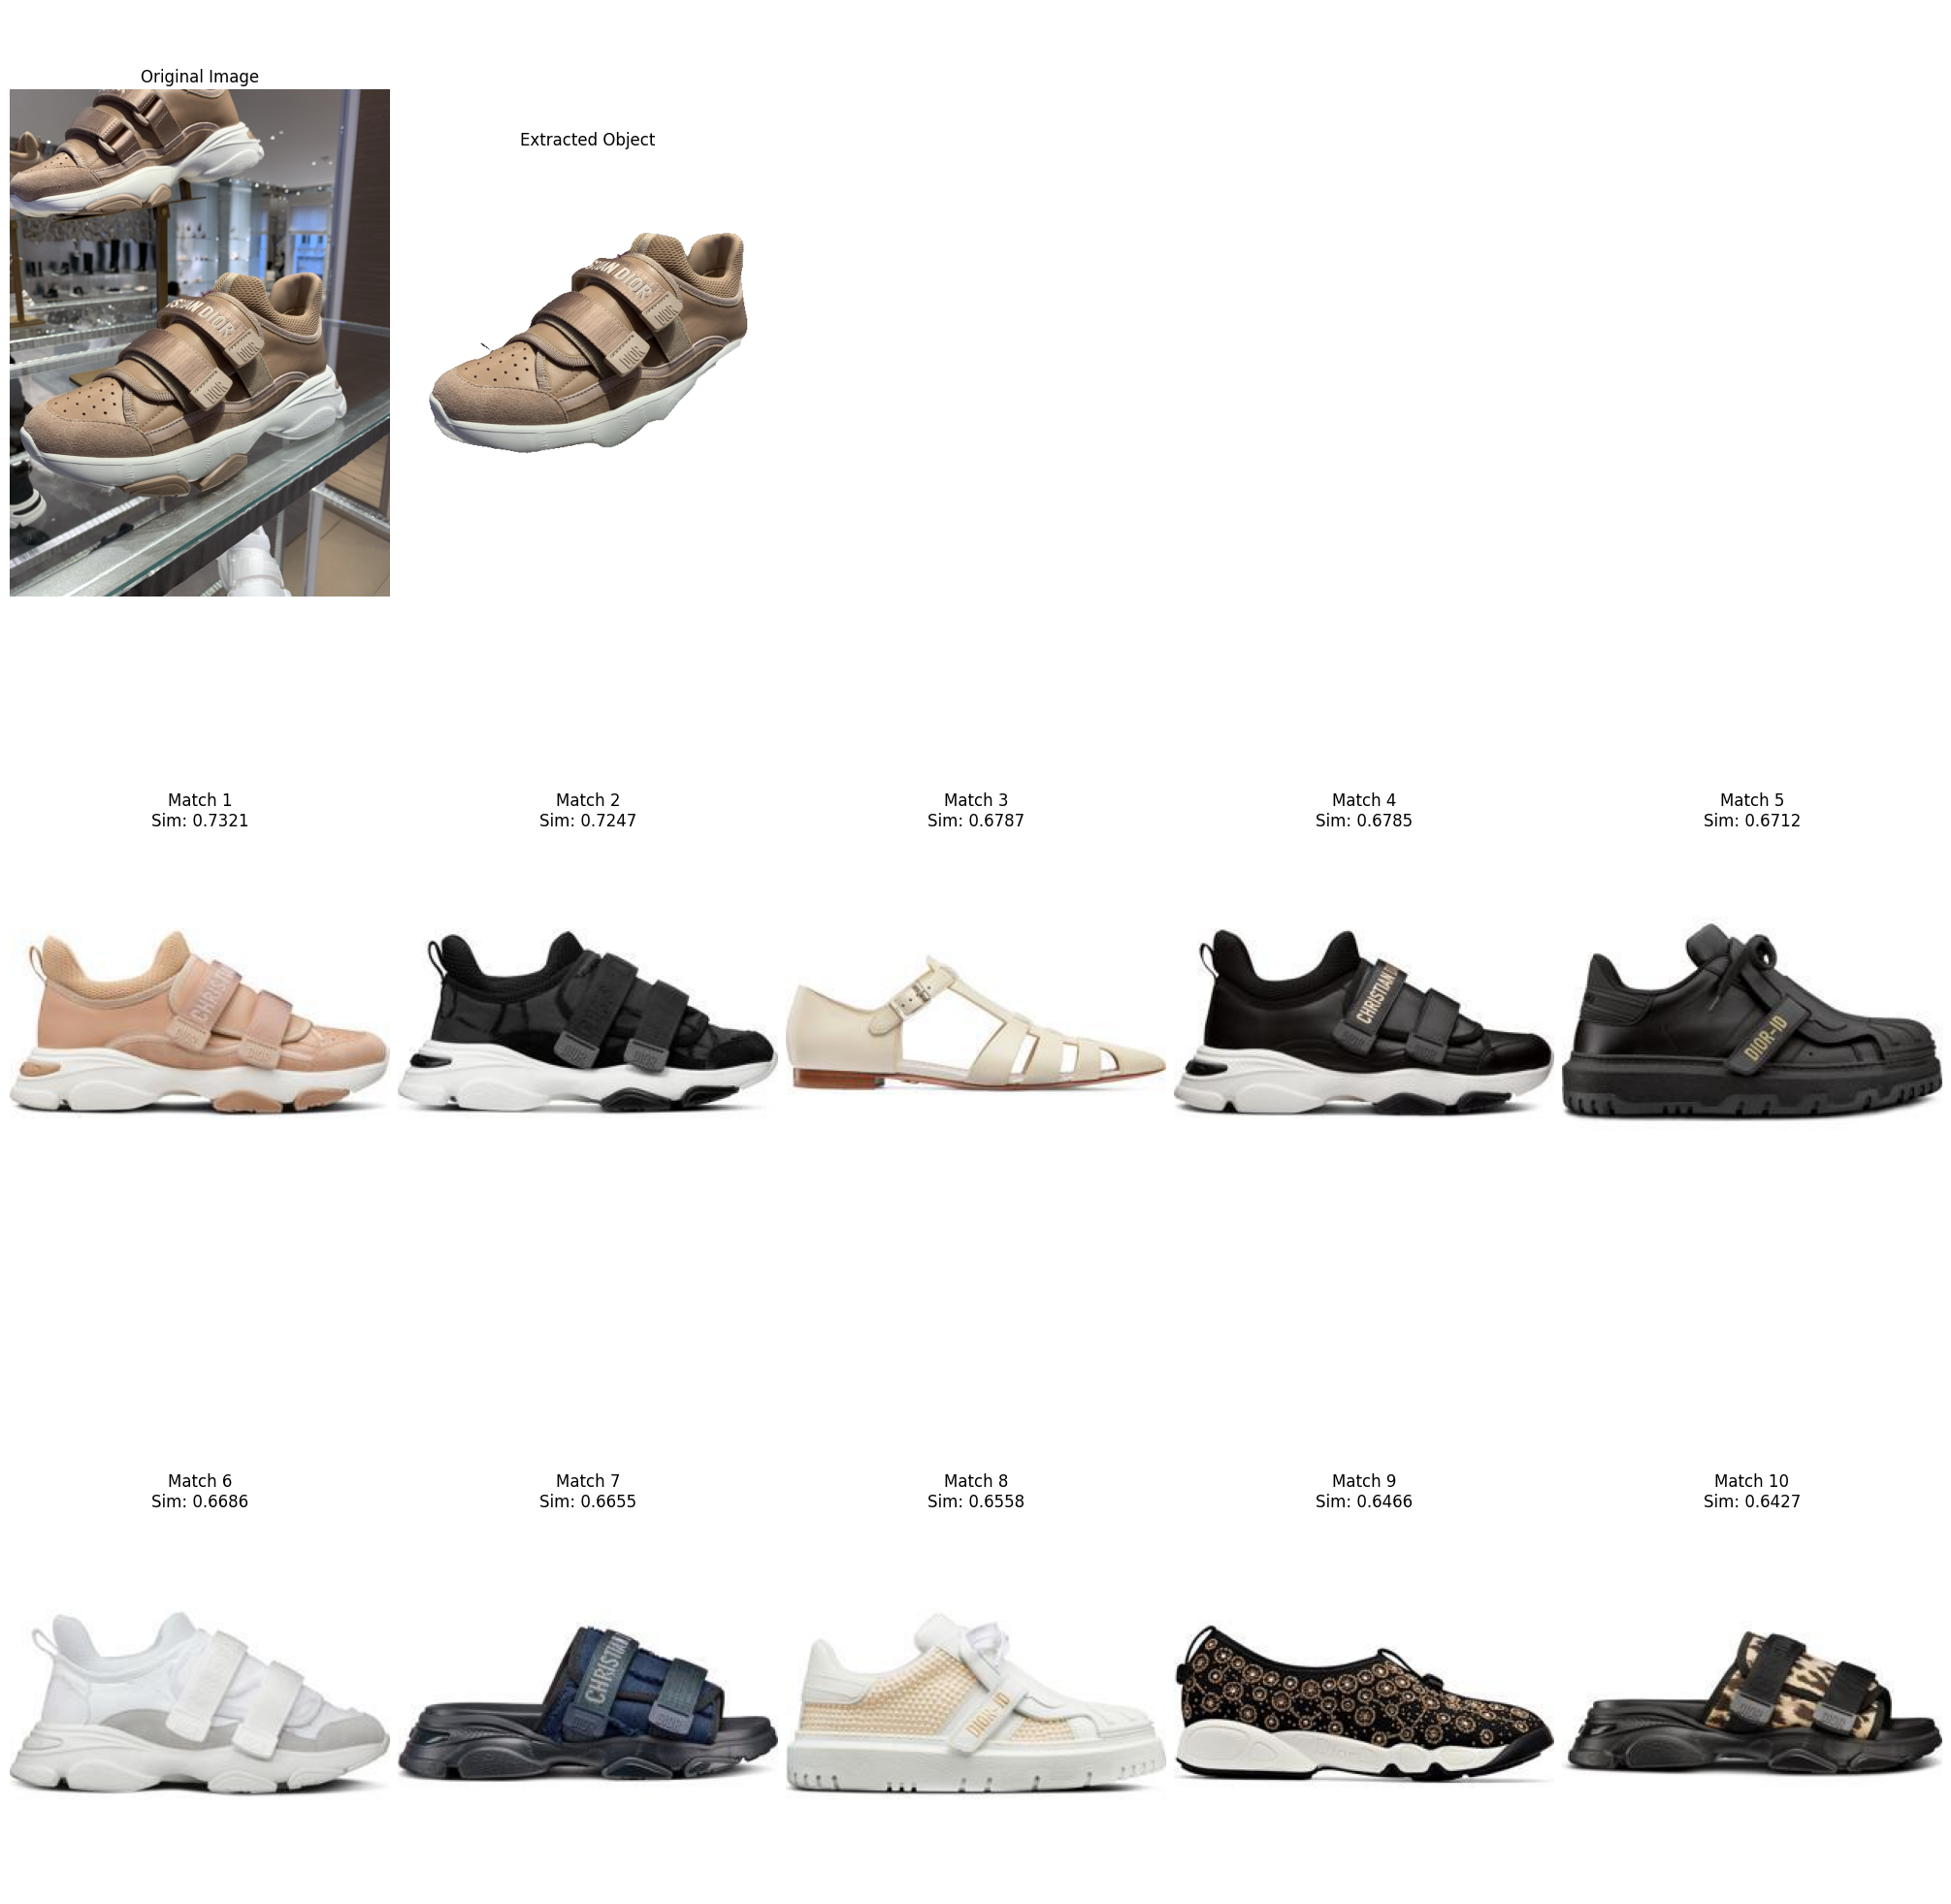
\includegraphics[width=\textwidth]{assets/good_classification.png}
    \caption{Example of a good classification result}
\end{figure}
\end{frame}

\begin{frame}{Bad Classification Example}
\begin{itemize}
    \item Challenges: reflections on the glass adversely affecting background removal and embeddings.
\end{itemize}
\begin{figure}
    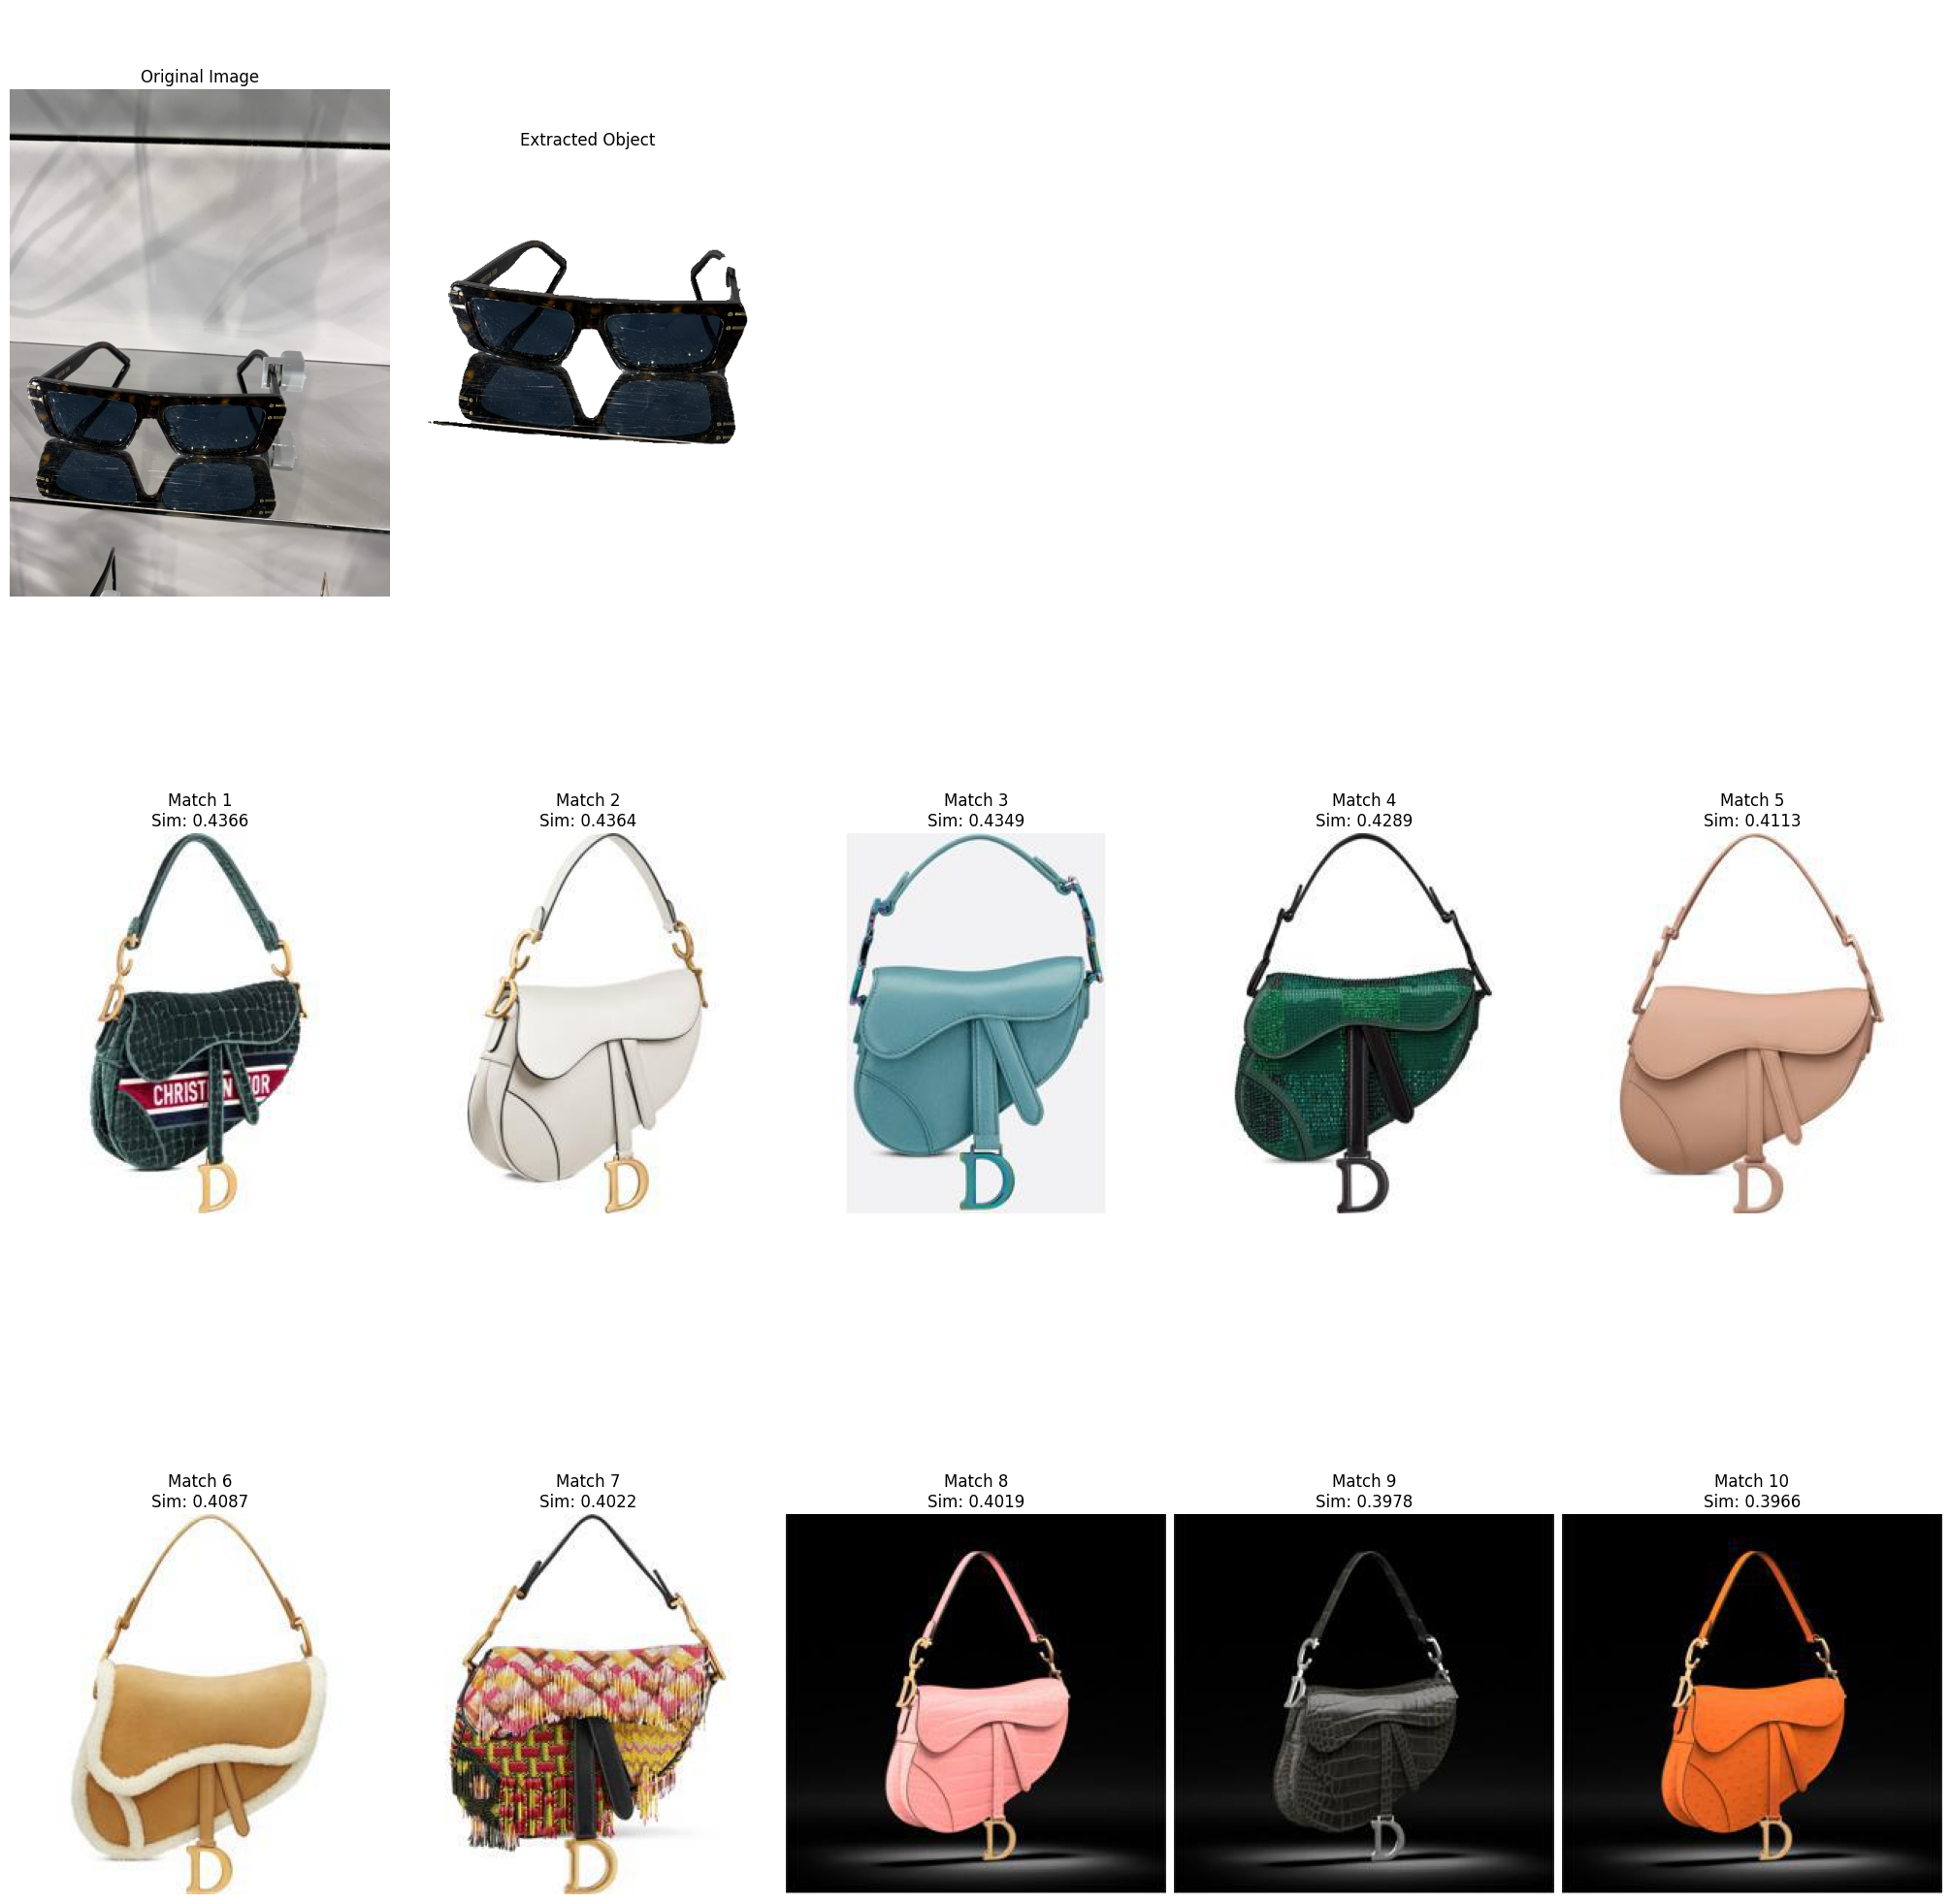
\includegraphics[width=\textwidth]{assets/bad_classification.png}
    \caption{Example of a bad classification due to reflections}
\end{figure}
\end{frame}

\section{Future Work}
\begin{frame}{Enhancing the Approach}
\begin{itemize}
    \item Use \textbf{TRELLIS} for generating 3D models and performing data augmentation with various object poses.
    \item Explore \textbf{Siamese Networks} to refine embeddings by focusing on important features.
\end{itemize}

\begin{columns}
    \column{0.5\textwidth}
    \begin{figure}
        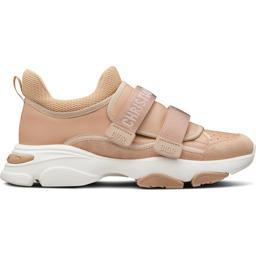
\includegraphics[width=0.65\textwidth]{assets/trellis_input.png}
        \caption{Input for TRELLIS}
    \end{figure}
    \column{0.5\textwidth}
    \begin{figure}
        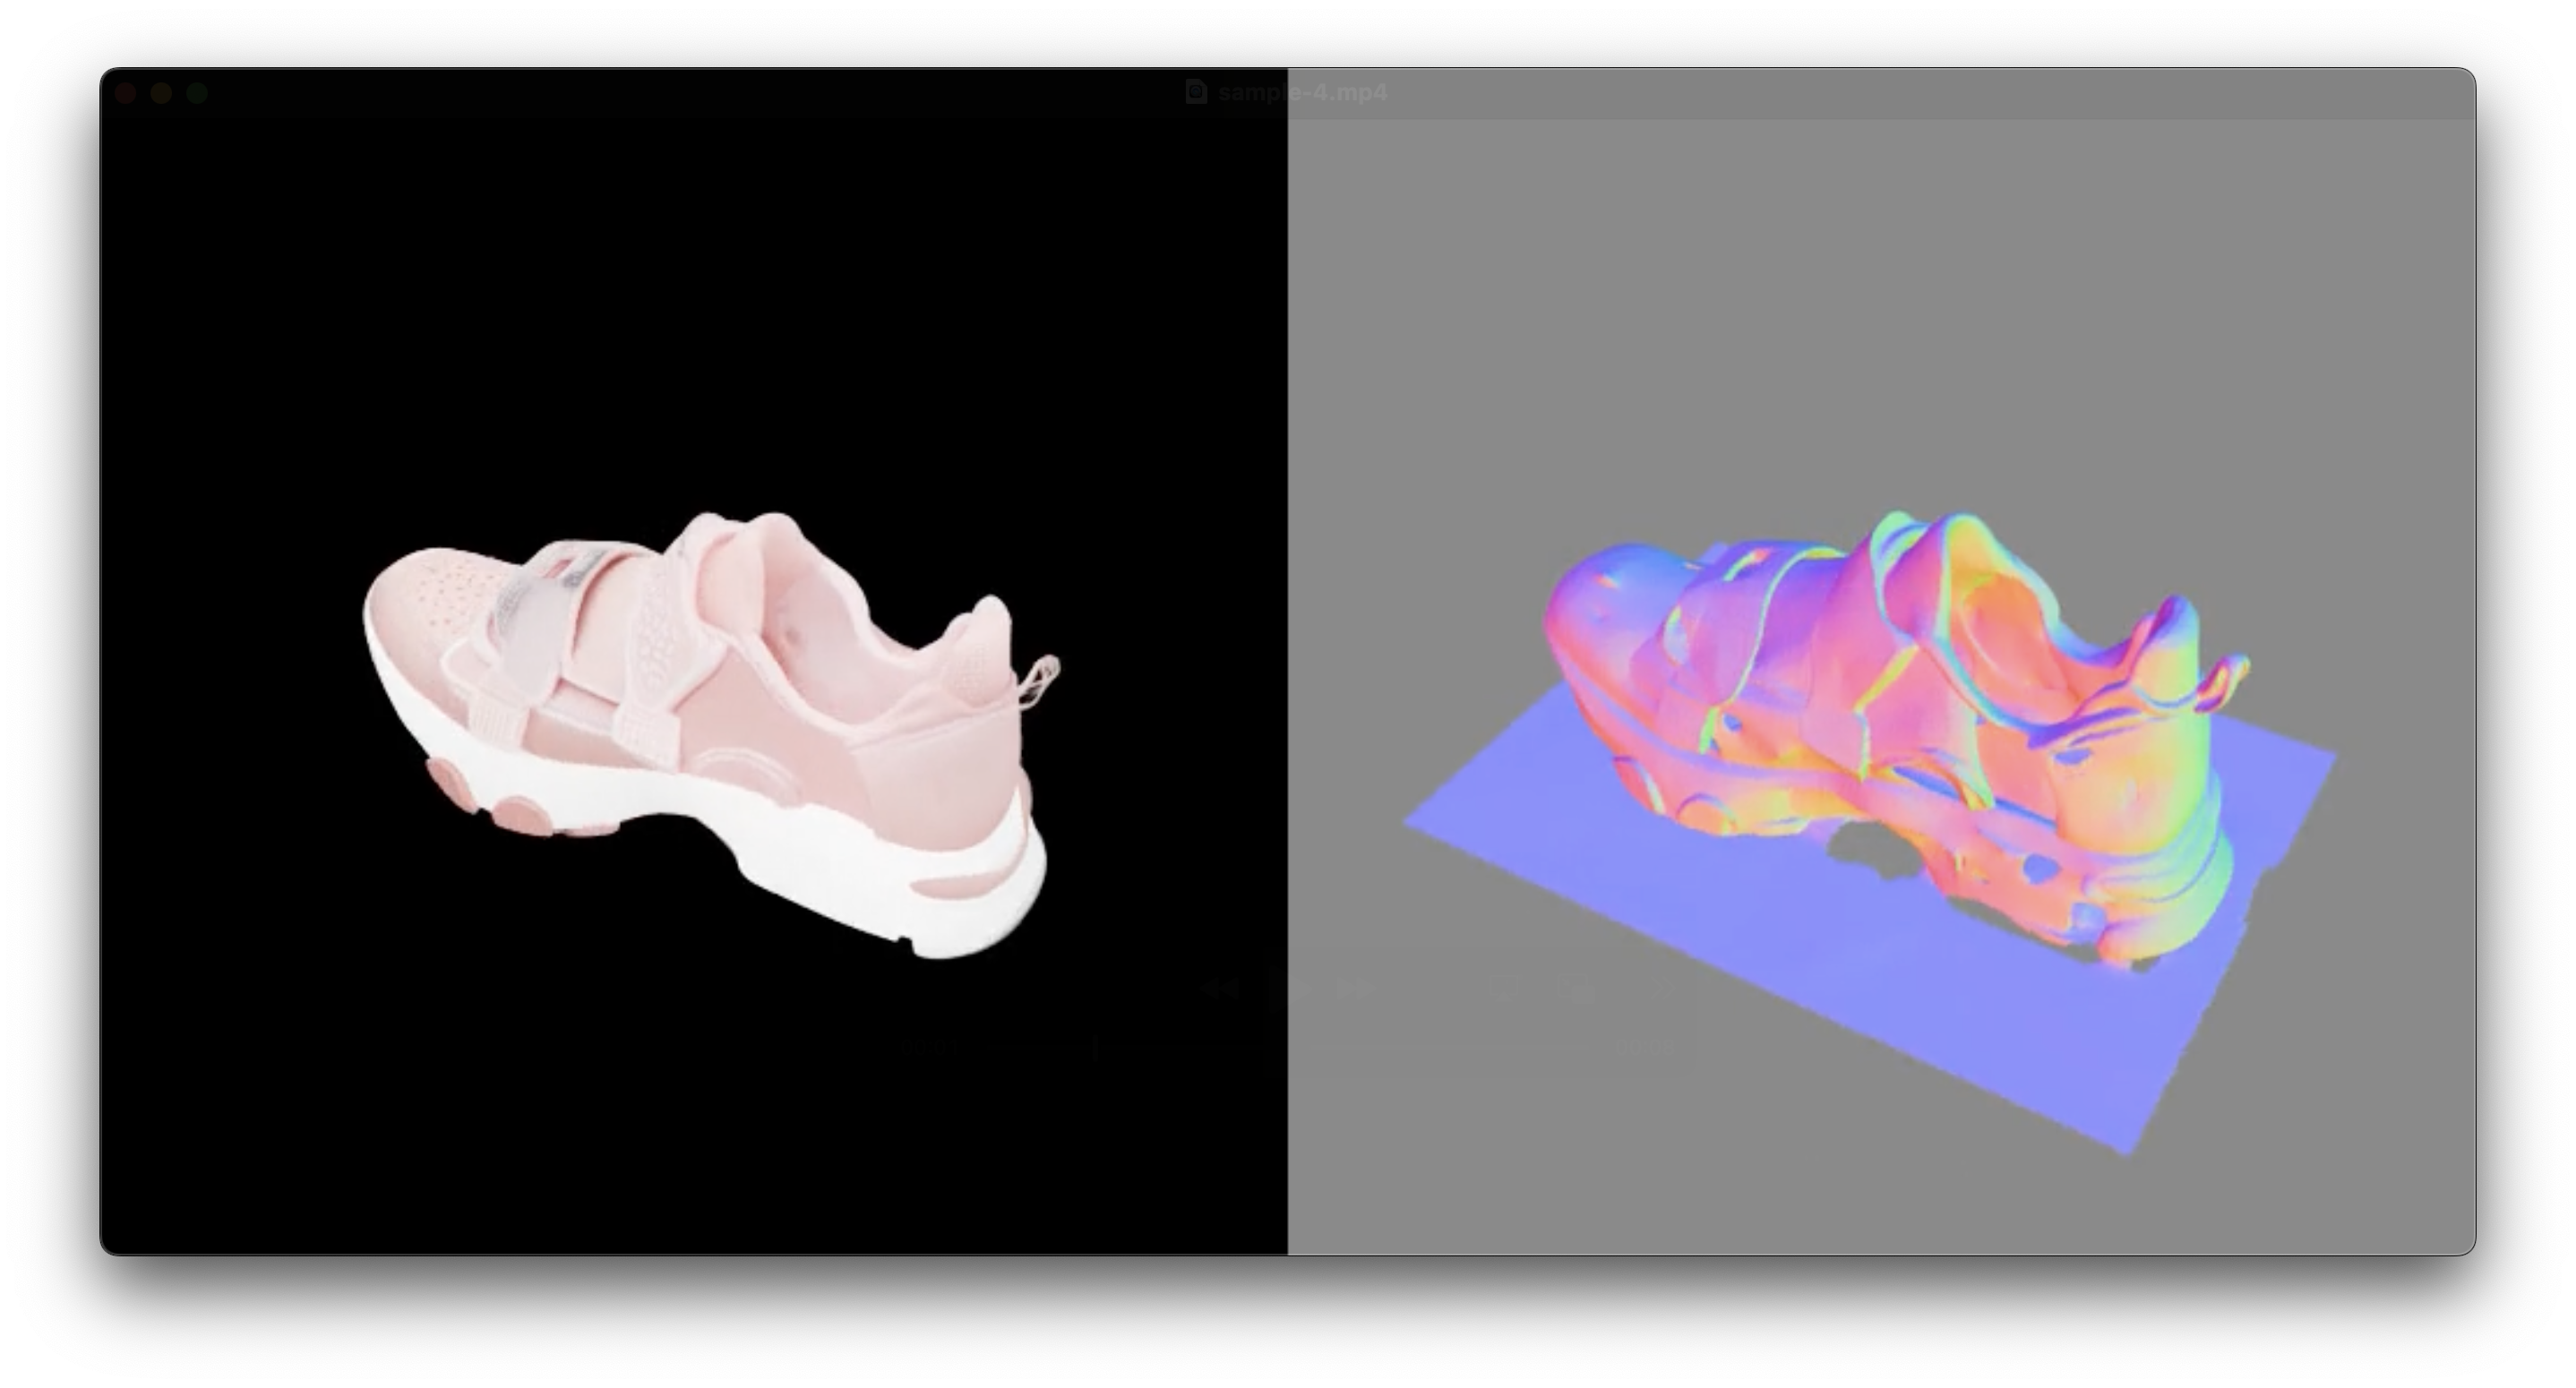
\includegraphics[width=1\textwidth]{assets/trellis_output.png}
        \caption{TRELLIS generated 3D model}
    \end{figure}
\end{columns}

\end{frame}

\section{User Interface}
\begin{frame}{Web Interface with Gradio}
\begin{itemize}
    \item Develop a quick UI using Gradio.
    \item Users can upload a picture and get top-X matches.
    \item This tool can aid in manual labeling and refine embeddings.
\end{itemize}
\end{frame}


\begin{frame}{ViTMSN Model}
\begin{itemize}
    \item Considering the ViTMSN approach for improved performance.
    \item Joint-embedding architecture from \emph{Masked Siamese Networks for Label-Efficient Learning}.
    \item Promising for low-shot and extreme low-shot regimes.
\end{itemize}
\end{frame}

\begin{frame}{Action Plan}
    \begin{itemize}
        \item \textbf{Focus 1: Evaluate Existing Models:} 
              Assess the performance of ResNet and ViT models with background removal preprocessing on the test set.
        \item \textbf{Focus 2: Data Augmentation:} 
              Create synthetic training images to enhance dataset diversity and size.
        \item \textbf{Focus 3: Classification Models:} 
              Experiment with and evaluate classification models to optimize prediction performance.
        \item \textbf{Focus 4: Multi-Object Classification:} 
              Develop methods to accurately classify and handle images containing multiple objects simultaneously.
    \end{itemize}
    \end{frame}

\section{NLP Approach}
    \begin{frame}{Using NLP for Image-to-Text and Matching}
    \begin{itemize}
        \item \textbf{Image-to-Text Conversion}:
        \begin{itemize}
            \item Generate descriptive captions for images to capture key attributes like color, material, and unique features.
        \end{itemize}
        \item \textbf{Text Embedding and Matching}:
        \begin{itemize}
            \item Convert captions into embeddings and store them in a vector database.
            \item Perform similarity search to find the closest matches to client-uploaded images.
        \end{itemize}
        \item \textbf{Combination with Image Embeddings}:
        \begin{itemize}
            \item This approach can be enhanced by combining text-based embeddings with image-based embeddings for improved accuracy.
        \end{itemize}
    \end{itemize}
\end{frame}

\begin{frame}{Improvement Attempt Using NLP}
    There are some challenging cases, with \textbf{color} or \textbf{texture}:
    \vspace{0.5cm} % Ajouter un espace vertical

    % Ajouter deux images côte à côte
% Ajouter une image à gauche et une description à droite
    \centering
    \begin{minipage}{0.5\textwidth}
        \centering
        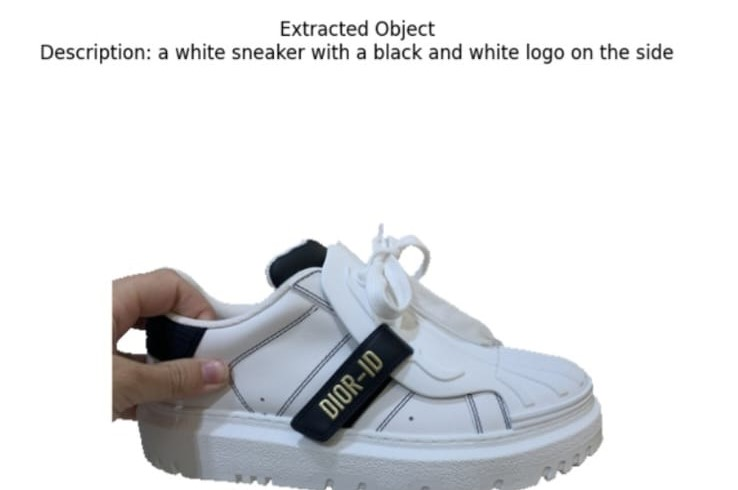
\includegraphics[width=\textwidth]{wrongColorShoes.jpg}
    \begin{figure}[h]
        \caption{Example: Color mismatch}
    \end{figure}
    \end{minipage}
    \hfill
    \begin{minipage}{0.45\textwidth}
        \raggedright
        \textbf{Blip Description:}
        \vspace{0.3cm} % Espacement entre le titre et la description
        \textit{"A white sneaker with a black and white logo on the side"}
    \end{minipage}
\end{frame}

\begin{frame}{Using NLP for Image-to-Text and Matching}

Steps : 
    \vspace{0.5cm} % Ajouter un espace vertical
    \begin{enumerate}
        \item Generate descriptions using the \textbf{BLIP model}.
        \item Convert descriptions into \textbf{text embeddings}.
        \item Combine \textbf{text embeddings} with 2D image embeddings and 3D-rendered image embeddings
        \item Use the \textbf{mean embedding} for improved matching.
    \end{enumerate}
\end{frame}

% Slide 3: Refining Results with Modern NLP Techniques
\section{Refining Results}
\begin{frame}{Improving Top-1 result}
    \begin{itemize}
        \item Use \textbf{more recent BLIP models} for better descriptions.
        \item Question prompt:
            \begin{quote}
                What is the object in this image? What is its color? What is its texture? What is a specific detail about it? \\
                Answer in the format: [object, color, texture, specificity].
            \end{quote}
        \end{itemize}

    \vspace{0.5cm}
    \textbf{Proposed Method}
    \begin{itemize}
        \item Select the top-5 DAM candidates selected after applying the cosine similarity on the embedding (without the BLIP embedding). 
        \item Apply BLIP to the top-5 and the test image to generate a structured description.
        \item Keep the candidate with the \textbf{highest overlap} in responses with the test image.
        \end{itemize}
\end{frame}

\end{document}
